% Options for packages loaded elsewhere
\PassOptionsToPackage{unicode}{hyperref}
\PassOptionsToPackage{hyphens}{url}
\PassOptionsToPackage{dvipsnames,svgnames,x11names}{xcolor}
%
\documentclass[
  ignorenonframetext,
]{beamer}
\usepackage{pgfpages}
\setbeamertemplate{caption}[numbered]
\setbeamertemplate{caption label separator}{: }
\setbeamercolor{caption name}{fg=normal text.fg}
\beamertemplatenavigationsymbolsempty
% Prevent slide breaks in the middle of a paragraph
\widowpenalties 1 10000
\raggedbottom
\setbeamertemplate{part page}{
  \centering
  \begin{beamercolorbox}[sep=16pt,center]{part title}
    \usebeamerfont{part title}\insertpart\par
  \end{beamercolorbox}
}
\setbeamertemplate{section page}{
  \centering
  \begin{beamercolorbox}[sep=12pt,center]{part title}
    \usebeamerfont{section title}\insertsection\par
  \end{beamercolorbox}
}
\setbeamertemplate{subsection page}{
  \centering
  \begin{beamercolorbox}[sep=8pt,center]{part title}
    \usebeamerfont{subsection title}\insertsubsection\par
  \end{beamercolorbox}
}
\AtBeginPart{
  \frame{\partpage}
}
\AtBeginSection{
  \ifbibliography
  \else
    \frame{\sectionpage}
  \fi
}
\AtBeginSubsection{
  \frame{\subsectionpage}
}
\usepackage{amsmath,amssymb}
\usepackage{lmodern}
\usepackage{iftex}
\ifPDFTeX
  \usepackage[T1]{fontenc}
  \usepackage[utf8]{inputenc}
  \usepackage{textcomp} % provide euro and other symbols
\else % if luatex or xetex
  \usepackage{unicode-math}
  \defaultfontfeatures{Scale=MatchLowercase}
  \defaultfontfeatures[\rmfamily]{Ligatures=TeX,Scale=1}
\fi
% Use upquote if available, for straight quotes in verbatim environments
\IfFileExists{upquote.sty}{\usepackage{upquote}}{}
\IfFileExists{microtype.sty}{% use microtype if available
  \usepackage[]{microtype}
  \UseMicrotypeSet[protrusion]{basicmath} % disable protrusion for tt fonts
}{}
\makeatletter
\@ifundefined{KOMAClassName}{% if non-KOMA class
  \IfFileExists{parskip.sty}{%
    \usepackage{parskip}
  }{% else
    \setlength{\parindent}{0pt}
    \setlength{\parskip}{6pt plus 2pt minus 1pt}}
}{% if KOMA class
  \KOMAoptions{parskip=half}}
\makeatother
\usepackage{xcolor}
\newif\ifbibliography
\usepackage{color}
\usepackage{fancyvrb}
\newcommand{\VerbBar}{|}
\newcommand{\VERB}{\Verb[commandchars=\\\{\}]}
\DefineVerbatimEnvironment{Highlighting}{Verbatim}{commandchars=\\\{\}}
% Add ',fontsize=\small' for more characters per line
\usepackage{framed}
\definecolor{shadecolor}{RGB}{248,248,248}
\newenvironment{Shaded}{\begin{snugshade}}{\end{snugshade}}
\newcommand{\AlertTok}[1]{\textcolor[rgb]{0.94,0.16,0.16}{#1}}
\newcommand{\AnnotationTok}[1]{\textcolor[rgb]{0.56,0.35,0.01}{\textbf{\textit{#1}}}}
\newcommand{\AttributeTok}[1]{\textcolor[rgb]{0.77,0.63,0.00}{#1}}
\newcommand{\BaseNTok}[1]{\textcolor[rgb]{0.00,0.00,0.81}{#1}}
\newcommand{\BuiltInTok}[1]{#1}
\newcommand{\CharTok}[1]{\textcolor[rgb]{0.31,0.60,0.02}{#1}}
\newcommand{\CommentTok}[1]{\textcolor[rgb]{0.56,0.35,0.01}{\textit{#1}}}
\newcommand{\CommentVarTok}[1]{\textcolor[rgb]{0.56,0.35,0.01}{\textbf{\textit{#1}}}}
\newcommand{\ConstantTok}[1]{\textcolor[rgb]{0.00,0.00,0.00}{#1}}
\newcommand{\ControlFlowTok}[1]{\textcolor[rgb]{0.13,0.29,0.53}{\textbf{#1}}}
\newcommand{\DataTypeTok}[1]{\textcolor[rgb]{0.13,0.29,0.53}{#1}}
\newcommand{\DecValTok}[1]{\textcolor[rgb]{0.00,0.00,0.81}{#1}}
\newcommand{\DocumentationTok}[1]{\textcolor[rgb]{0.56,0.35,0.01}{\textbf{\textit{#1}}}}
\newcommand{\ErrorTok}[1]{\textcolor[rgb]{0.64,0.00,0.00}{\textbf{#1}}}
\newcommand{\ExtensionTok}[1]{#1}
\newcommand{\FloatTok}[1]{\textcolor[rgb]{0.00,0.00,0.81}{#1}}
\newcommand{\FunctionTok}[1]{\textcolor[rgb]{0.00,0.00,0.00}{#1}}
\newcommand{\ImportTok}[1]{#1}
\newcommand{\InformationTok}[1]{\textcolor[rgb]{0.56,0.35,0.01}{\textbf{\textit{#1}}}}
\newcommand{\KeywordTok}[1]{\textcolor[rgb]{0.13,0.29,0.53}{\textbf{#1}}}
\newcommand{\NormalTok}[1]{#1}
\newcommand{\OperatorTok}[1]{\textcolor[rgb]{0.81,0.36,0.00}{\textbf{#1}}}
\newcommand{\OtherTok}[1]{\textcolor[rgb]{0.56,0.35,0.01}{#1}}
\newcommand{\PreprocessorTok}[1]{\textcolor[rgb]{0.56,0.35,0.01}{\textit{#1}}}
\newcommand{\RegionMarkerTok}[1]{#1}
\newcommand{\SpecialCharTok}[1]{\textcolor[rgb]{0.00,0.00,0.00}{#1}}
\newcommand{\SpecialStringTok}[1]{\textcolor[rgb]{0.31,0.60,0.02}{#1}}
\newcommand{\StringTok}[1]{\textcolor[rgb]{0.31,0.60,0.02}{#1}}
\newcommand{\VariableTok}[1]{\textcolor[rgb]{0.00,0.00,0.00}{#1}}
\newcommand{\VerbatimStringTok}[1]{\textcolor[rgb]{0.31,0.60,0.02}{#1}}
\newcommand{\WarningTok}[1]{\textcolor[rgb]{0.56,0.35,0.01}{\textbf{\textit{#1}}}}
\usepackage{graphicx}
\makeatletter
\def\maxwidth{\ifdim\Gin@nat@width>\linewidth\linewidth\else\Gin@nat@width\fi}
\def\maxheight{\ifdim\Gin@nat@height>\textheight\textheight\else\Gin@nat@height\fi}
\makeatother
% Scale images if necessary, so that they will not overflow the page
% margins by default, and it is still possible to overwrite the defaults
% using explicit options in \includegraphics[width, height, ...]{}
\setkeys{Gin}{width=\maxwidth,height=\maxheight,keepaspectratio}
% Set default figure placement to htbp
\makeatletter
\def\fps@figure{htbp}
\makeatother
\setlength{\emergencystretch}{3em} % prevent overfull lines
\providecommand{\tightlist}{%
  \setlength{\itemsep}{0pt}\setlength{\parskip}{0pt}}
\setcounter{secnumdepth}{-\maxdimen} % remove section numbering
\usepackage{graphicx}
\usepackage{bm}
\usepackage{amsthm}
\usepackage{amsmath}
\usepackage{amsfonts}
\usepackage{amscd}
\usepackage{amssymb}
\usepackage{natbib}
\usepackage{url}
\usepackage{tikz}
\definecolor{foreground}{RGB}{255,255,255}
\definecolor{background}{RGB}{34,28,54}
\definecolor{title}{RGB}{105,165,255}
\definecolor{gray}{RGB}{175,175,175}
\definecolor{lightgray}{RGB}{225,225,225}
\definecolor{subtitle}{RGB}{232,234,255}
\definecolor{hilight}{RGB}{112,224,255}
\definecolor{vhilight}{RGB}{255,111,207}
\setbeamertemplate{footline}[page number]
\ifLuaTeX
  \usepackage{selnolig}  % disable illegal ligatures
\fi
\IfFileExists{bookmark.sty}{\usepackage{bookmark}}{\usepackage{hyperref}}
\IfFileExists{xurl.sty}{\usepackage{xurl}}{} % add URL line breaks if available
\urlstyle{same} % disable monospaced font for URLs
\hypersetup{
  pdftitle={STAT 528 - Advanced Regression Analysis II},
  pdfauthor={Variance Reduction: Envelope Model},
  colorlinks=true,
  linkcolor={Maroon},
  filecolor={Maroon},
  citecolor={Blue},
  urlcolor={blue},
  pdfcreator={LaTeX via pandoc}}

\title{STAT 528 - Advanced Regression Analysis II}
\author{Variance Reduction: Envelope Model}
\date{}
\institute{Daniel J. Eck\\
Department of Statistics\\
University of Illinois}

\begin{document}
\frame{\titlepage}

\begin{frame}
\newcommand{\Var}{\mathrm{Var}}
\newcommand{\Prob}{\mathbb{P}}
\newcommand{\R}{\mathbb{R}}
\newcommand{\E}{\mathrm{E}}
\newcommand{\Y}{\mathbb{Y}}
\newcommand{\X}{\mathbb{X}}
\end{frame}

\begin{frame}{Learning Objectives Today}
\protect\hypertarget{learning-objectives-today}{}
\begin{itemize}
\tightlist
\item
  Multivariate regression modeling
\item
  Variance reduction via envelope
\item
  Dimension selection robustness
\end{itemize}
\end{frame}

\begin{frame}{Example: wheat protein}
\protect\hypertarget{example-wheat-protein}{}
This data contains measurements on protein content and the logarithms of
near-infrared reflectance at six wavelengths across the range 1680-2310
nm measured on each of \(n = 50\) samples of ground wheat.

We will:

\begin{itemize}
\tightlist
\item
  consider an analysis of the first two responses \((Y_1,Y_2)\)
\item
  convert the continuous measure of protein content into a categorical
  variable indicating low and high levels of protein
\end{itemize}

Here, the mean difference, \(\mu_2 - \mu_1\) corresponds to \(\beta\) in
the model \[
  Y = \alpha + \beta X + \varepsilon
\] where \(X = 0\) indicates a high level of protein and \(X = 1\)
indicates a low level of protein.

Interest is in whether changes in protein concentration are detectable.
\end{frame}

\begin{frame}[fragile]{}
\protect\hypertarget{section}{}
This data set is in the \texttt{Renvlp} package. We now load in the
data.

\vspace{12pt}
\tiny

\begin{Shaded}
\begin{Highlighting}[]
\FunctionTok{library}\NormalTok{(Renvlp)}
\FunctionTok{library}\NormalTok{(tidyverse)}
\FunctionTok{library}\NormalTok{(ggplot2)}
\FunctionTok{library}\NormalTok{(reshape2)}
\FunctionTok{data}\NormalTok{(wheatprotein)}

\NormalTok{dat }\OtherTok{\textless{}{-}} \FunctionTok{data.frame}\NormalTok{(}\AttributeTok{Y1 =}\NormalTok{ wheatprotein[, }\DecValTok{1}\NormalTok{] }\SpecialCharTok{{-}} \FunctionTok{mean}\NormalTok{( wheatprotein[, }\DecValTok{1}\NormalTok{]), }
                  \AttributeTok{Y2 =}\NormalTok{ wheatprotein[, }\DecValTok{2}\NormalTok{] }\SpecialCharTok{{-}} \FunctionTok{mean}\NormalTok{( wheatprotein[, }\DecValTok{2}\NormalTok{]),}
                  \AttributeTok{X  =}\NormalTok{ wheatprotein[, }\DecValTok{8}\NormalTok{])}
\NormalTok{dat}\SpecialCharTok{$}\NormalTok{X }\OtherTok{\textless{}{-}} \FunctionTok{as.factor}\NormalTok{(dat}\SpecialCharTok{$}\NormalTok{X)}
\FunctionTok{head}\NormalTok{(dat)}
\end{Highlighting}
\end{Shaded}

\begin{verbatim}
##       Y1    Y2 X
## 1  -6.16  -6.8 0
## 2 -16.16 -17.8 0
## 3 -17.16 -11.8 1
## 4 -24.16 -14.8 1
## 5 -10.16 -10.8 1
## 6  24.84  17.2 0
\end{verbatim}
\end{frame}

\begin{frame}[fragile]{}
\protect\hypertarget{section-1}{}
We will now consider an envelope model with \(\hat{u} = 1\):

\vspace{12pt}
\tiny

\begin{Shaded}
\begin{Highlighting}[]
\FunctionTok{u.env}\NormalTok{(}\AttributeTok{X =} \FunctionTok{as.numeric}\NormalTok{(dat}\SpecialCharTok{$}\NormalTok{X), }\AttributeTok{Y =}\NormalTok{ dat[, }\DecValTok{1}\SpecialCharTok{:}\DecValTok{2}\NormalTok{])}
\end{Highlighting}
\end{Shaded}

\begin{verbatim}
## $u.aic
## [1] 1
## 
## $u.bic
## [1] 1
## 
## $u.lrt
## [1] 1
## 
## $loglik.seq
## [1] -383.5512 -364.3534 -364.1719
## 
## $aic.seq
## [1] 777.1024 740.7067 742.3438
## 
## $bic.seq
## [1] 786.6625 752.1788 755.7279
\end{verbatim}

\begin{Shaded}
\begin{Highlighting}[]
\CommentTok{\# ratios at u = 1}
\NormalTok{env\_mod }\OtherTok{\textless{}{-}} \FunctionTok{env}\NormalTok{(}\AttributeTok{X =} \FunctionTok{as.numeric}\NormalTok{(dat}\SpecialCharTok{$}\NormalTok{X), }\AttributeTok{Y =}\NormalTok{ dat[, }\DecValTok{1}\SpecialCharTok{:}\DecValTok{2}\NormalTok{], }\AttributeTok{u =} \DecValTok{1}\NormalTok{)}
\NormalTok{env\_mod}\SpecialCharTok{$}\NormalTok{ratio}
\end{Highlighting}
\end{Shaded}

\begin{verbatim}
##          [,1]
## [1,] 28.40504
## [2,] 19.23553
\end{verbatim}
\end{frame}

\begin{frame}{}
\protect\hypertarget{section-2}{}
We now visualize the distribution of measurements of wheat protein with
an emphasis on the distinction between measurements in the high and low
protein groups:

\vspace{12pt}

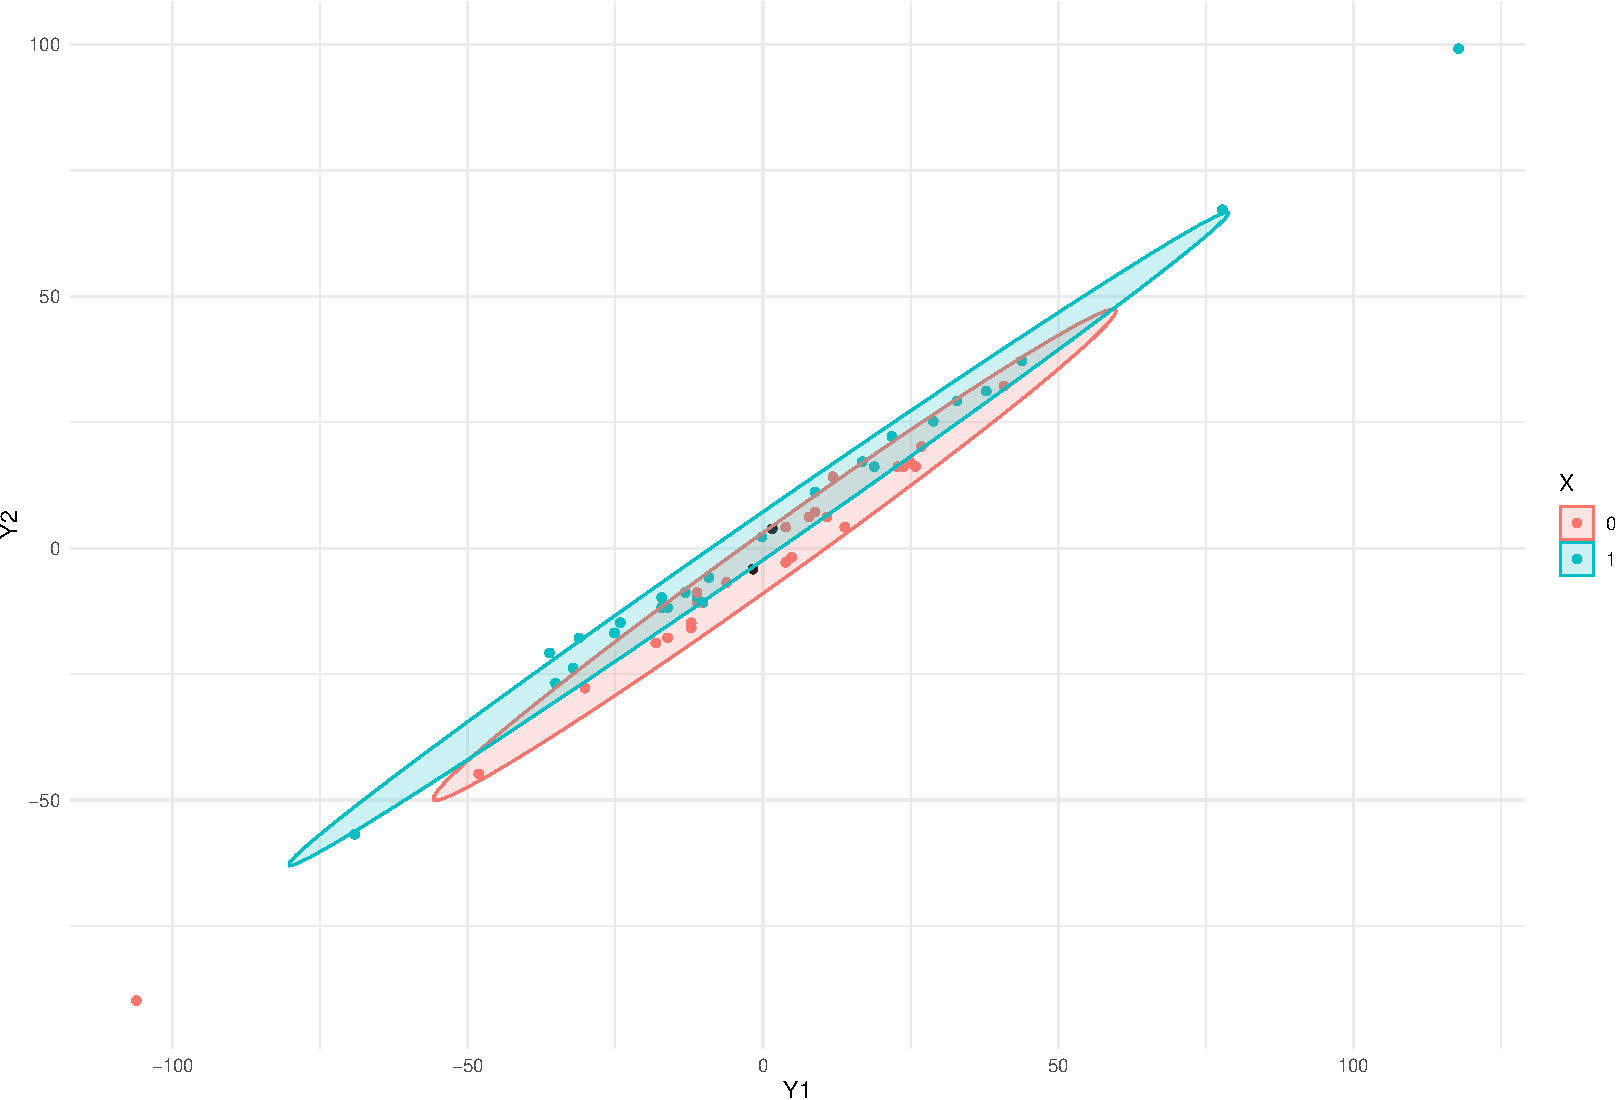
\includegraphics{week15_p2_files/figure-beamer/unnamed-chunk-3-1.pdf}
\end{frame}

\begin{frame}{}
\protect\hypertarget{section-3}{}
We add the envelope subspace to the previous plot.

\vspace{12pt}

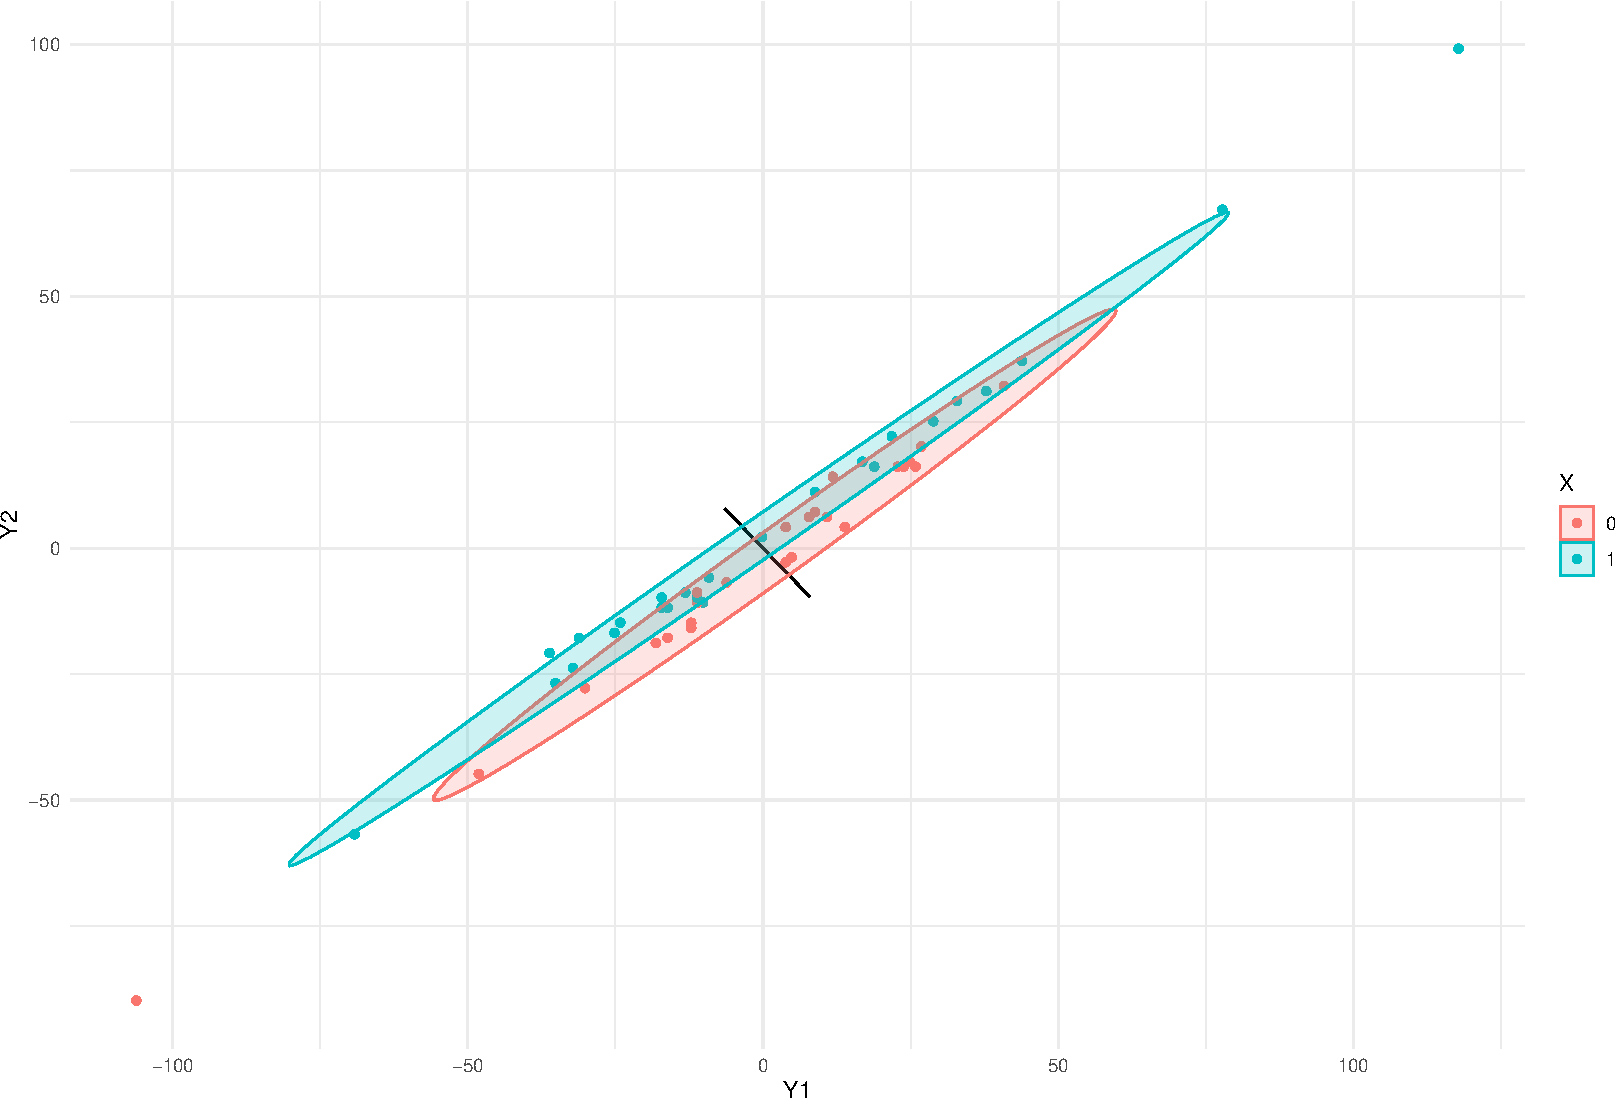
\includegraphics{week15_p2_files/figure-beamer/unnamed-chunk-4-1.pdf}
\end{frame}

\begin{frame}[fragile]{Robustness to dimension selection variability}
\protect\hypertarget{robustness-to-dimension-selection-variability}{}
We can use the \texttt{weighted.env} function to estimation the
variability of the weighted envelope estimator in the wheat protein
example.

We see that meaningful variance reduction is still observed when we
account for model selection variance.

\vspace{12pt}
\tiny

\begin{Shaded}
\begin{Highlighting}[]
\FunctionTok{set.seed}\NormalTok{(}\DecValTok{13}\NormalTok{)}
\FunctionTok{system.time}\NormalTok{(}
\NormalTok{  wtenv }\OtherTok{\textless{}{-}} \FunctionTok{weighted.env}\NormalTok{(}\AttributeTok{X =} \FunctionTok{as.numeric}\NormalTok{(dat}\SpecialCharTok{$}\NormalTok{X), }\AttributeTok{Y =}\NormalTok{ dat[, }\DecValTok{1}\SpecialCharTok{:}\DecValTok{2}\NormalTok{], }\AttributeTok{bstrpNum =} \FloatTok{1e3}\NormalTok{))}
\end{Highlighting}
\end{Shaded}

\begin{verbatim}
##    user  system elapsed 
##   2.878   0.015   2.894
\end{verbatim}

\begin{Shaded}
\begin{Highlighting}[]
\DocumentationTok{\#\# ratios wrt to weighted envelope estimator after bootstrapping}
\NormalTok{wtenv}\SpecialCharTok{$}\NormalTok{ratios}
\end{Highlighting}
\end{Shaded}

\begin{verbatim}
##          [,1]
## [1,] 2.334444
## [2,] 2.333241
\end{verbatim}
\end{frame}

\begin{frame}[fragile]{}
\protect\hypertarget{section-4}{}
However, these efficiency gains are lower than an analysis that assumes
\(u = 1\). Whether such an assumption holds is unknown.

\vspace{12pt}
\tiny

\begin{Shaded}
\begin{Highlighting}[]
\OtherTok{\#\# ratios wrt to weighted envelope estimator after bootstrapping}
\NormalTok{wtenv$ratios}

\OtherTok{\#\# ratios conditional on u = 1}
\NormalTok{env\_mod$ratio}

\OtherTok{\#\# number of times each dimension is selected}
\NormalTok{wtenv$bic\_select}
\end{Highlighting}
\end{Shaded}
\end{frame}

\end{document}
